\section{Spin Sorting}

Each of the bunches in the two RHIC beams is polarized independently, and the
polarization pattern can change from fill to fill. An accurate record of the
spin state of each bunch crossing in a fill is essential for any spin
analysis. The polarization pattern for the rings is set by the RHIC
Collider-Accelerator Department (C-AD) and broadcast through the CDEV
\cite{Barton:2003sh} control and monitoring system. The pattern is formatted
as a list of 360 8 bit numbers, one for each of the time buckets in RHIC, and
is defined in terms of the bunch crossings at the 12 o'clock position in the
RHIC ring. The beam experiences an odd number of spin flips in between 12
o'clock and the STAR IP at six o'clock, so the beam polarizations at STAR are
flipped relative to the broadcast record. The interpretation of each bit is
given in Table \ref{tbl:spin8}.

\begin{table}
  \begin{center}
  % \begin{ruledtabular}
    \begin{tabular}{c|l}
      \hline
      bit & meaning \\
      \hline
      \hline
      0 & yellow beam filled\\
      \hline
      1 & yellow beam polarized up\\
      \hline
      2 & yellow beam polarized down\\
      \hline
      3 & yellow beam unpolarized\\
      \hline
      4 & blue beam filled\\
      \hline
      5 & blue beam polarized up\\
      \hline
      6 & blue beam polarized down\\
      \hline
      7 & blue beam unpolarized\\
      \hline
    \end{tabular}
  % \end{ruledtabular}
  \end{center}
  \caption{Significance of each of the bits in an eight bit spin record.}
  \label{tbl:spin8}
\end{table}

A given bunch from the Blue ring always collides with the same bunch from the
Yellow ring at a specific interaction point in the RHIC ring over the course
of a fill. C-AD has historically configured the beams so that bunch zero from
the Blue beam collides with bunch zero from the Yellow beam at the PHENIX IP,
and as a result the PHENIX experiment sees only one abort gap in its fill
patterns. The situation is different at STAR, where the RHIC ``toggle mode''
defines the pairs of bunches from the Blue and Yellow beams that collide. The
toggle mode is typically set once at the beginning of the RHIC data-taking
period, and is encoded implicitly in the spin patterns broadcast by CDEV.

After accounting for the spin flip and the toggle mode, an analysis must map
the event IDs recorded at the experiment to the 7 bit bunch crossing IDs
defined by CDEV in order to determine the spin state of a given event. The
STAR Trigger receives this information from RHIC for every event, but analyses
have observed occasional inaccuracies in the feed that render it unreliable.
Instead, STAR uses a more robust 48 bit counter synchronized to the 9.4 MHz
RHIC clock to uniquely identify every event. The 7 bit bunch crossing IDs can
be expressed in terms of this 48 bit counter as
%
\begin{equation}
  \mathrm{7~bit~ID} = \left(\mathrm{48~bit~counter} + \mathrm{offset}\right)~mod~120
\end{equation}
%
The offset is calculated for each STAR run by generating 120 histograms of
triggers versus the 7 bit bunch IDs for each possible value of the offset,
comparing these histograms to a histogram of the intended spin pattern at
STAR, and searching for a minimum in the $\chi^2$ distribution. An example of
the overlap between the trigger rate versus bunch crossing ID and the spin
pattern after the correct offset has been applied is shown in Figure
\ref{fig:bxing-offset}. The offsets for each STAR run are calculated once and
uploaded to the STAR Calibrations DB which allows them to be applied by all
STAR spin analyses. Further details of the spin state determination can be
found in Reference \cite{spin-db-website}.

\begin{figure}
  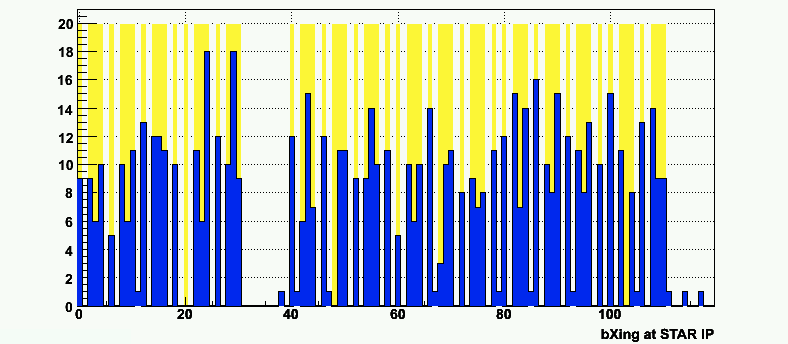
\includegraphics[width=1.0\textwidth]{figures/bxing-offset-determined}
  \caption{Distribution of events (blue) versus the corrected 7 bit bunch
  crossing IDs at the STAR interaction point. The yellow bars indicate the
  bunch crossings where both beams have filled bunches according to the
  intended spin patterns broadcast by CDEV.}
  \label{fig:bxing-offset}
\end{figure}
